\section{Specific Challenges of RS Data}
\label{sec:rs_challenges}
The application of computer vision techniques, originally developed for natural optical imagery, to RS data presents a number of domain-specific challenges. 

\begin{figure}[t]
    \centering
    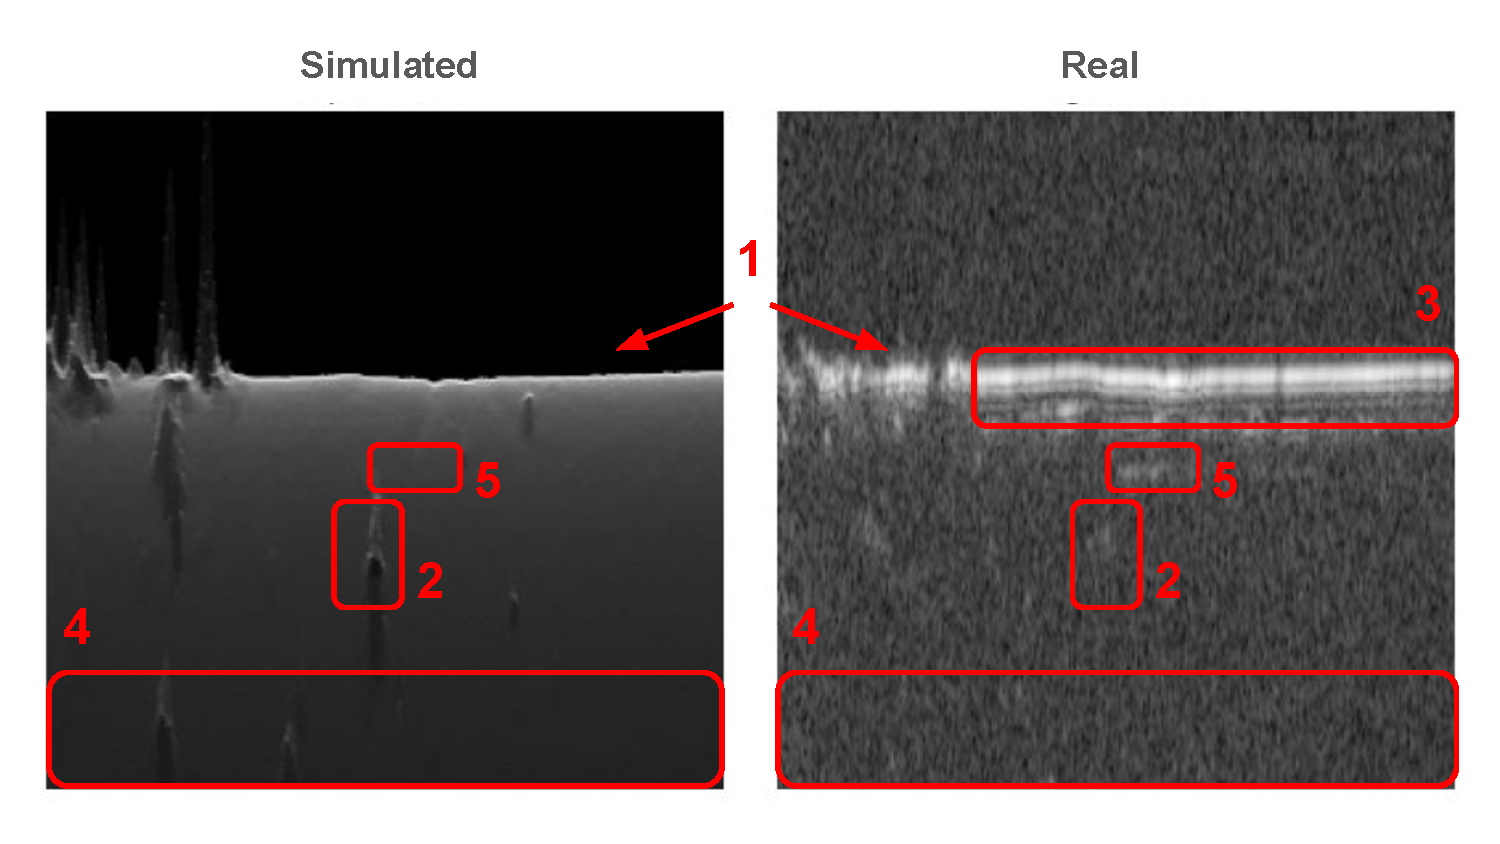
\includegraphics[width=\linewidth]{images/sim_real_radargram_annotated}
    \caption{Example of a simulated (left) and real (right) radargram patch from the Elysium Planitia study region, with key features and challenges highlighted. 
    (1) The bright surface return is clearly visible in both cases, though it appears more diffuse in the real data due to speckle noise and surface roughness. 
    (2) An isolated clutter point, correctly predicted and sharply rendered in the simulated radargram, is present in the real data but is strongly suppressed and corrupted by overwhelming thermal noise, demonstrating the challenge of isolating clutter from useful signal. 
    (3) In the real radargram, two shallow reflectors closely following the surface profile suggest the presence of thin stratified subsurface layers near the surface, which are not captured in the topography-based simulation. 
    (4) At greater depths, the simulated radargram still contains weak clutter-like echoes from surface features, whereas the corresponding region in the real data is dominated by noise and signal attenuation, illustrating the combined effect of attenuation and limited sensitivity to deep interfaces.
    (5) A distinct subsurface reflector is visible in the real radargram. Crucially, this real geological structure is \textit{completely absent} in the simulation, as the latter models only surface-related echoes. Identifying such un-modeled features represents a core objective of this work, validated by their absence in the simulated baseline.}
    \label{fig:rs_challenges_sim_real}
\end{figure}

Radargrams exhibit physical and statistical properties that differ significantly from those of conventional (RGB) images and are affected by several sources of signal degradation:
\begin{itemize}
    \item \textbf{Signal Attenuation:} Radar signals attenuate approximately exponentially with depth as they propagate through lossy dielectric media. Consequently, deep interfaces appear with much lower amplitude than shallow reflectors and are often embedded in a background close to the noise floor. Time-varying gain functions are commonly applied to partially compensate this effect, but they also amplify unwanted noise.
    \item \textbf{Speckle Noise:} As a coherent imaging system, an RS is subject to multiplicative speckle, a granular noise arising from the constructive and destructive interference of scattered waves within each resolution cell. Speckle can obscure fine stratigraphic details, reduce the effective signal-to-noise ratio (SNR), and strongly degrade standard edge and texture-based descriptors.
    \item \textbf{Surface Clutter:} Off-nadir reflections from topographic features (e.g., crater rims, scarps, rough volcanic terrains) can arrive with the same time delay as nadir subsurface echoes (see acquisition geometry in Fig.~\ref{fig:rs_geometry_clutter}). These clutter contributions generate apparent reflectors in the radargram that do not correspond to real subsurface interfaces, complicating the discrimination between clutter and true subsurface structure. This discrimination is one of the central objectives of the methods developed in this thesis.
    \item \textbf{Instrumental Noise:} In addition to speckle and clutter, RS data are affected by receiver thermal noise, quantization noise, radio-frequency interference, and, for low-frequency systems, by contributions from galactic background emission. These components raise the effective noise floor and may introduce localized artefacts that further reduce the visibility of weak subsurface echoes.
    \item \textbf{Galactic and Ionospheric Emission:} For low-frequency systems, such as those operating in the HF/VHF bands, sky noise from galactic background emission and ionospheric disturbances can substantially contribute to the received signal, further degrading sensitivity to faint subsurface targets and introducing temporal variability that is difficult to model.
    \item \textbf{Wide Dynamic Range:} Radar echoes span a very wide dynamic range in power (often tens of dB), from strong surface returns to faint deep signals. Representing and processing such data without saturating bright echoes or burying weak reflectors is non-trivial and requires carefully designed pre-processing and normalization steps, as discussed in Chapter~\ref{cha:methodology}.
\end{itemize}

These factors jointly make the automatic analysis of radargrams substantially more challenging than that of natural images, and motivate the development of processing pipelines and learning models that explicitly account for the underlying radar physics and noise characteristics, rather than relying on naive assumptions about image statistics.
In most practical scenarios, including the SHARAD data used in this thesis, radargrams are obtained after classical range and azimuth compression steps, which coherently integrate the received echoes to enhance the SNR and improve range and along-track resolution~\cite{yebasse2025advances}.
Nonetheless, significant residual speckle, clutter, and instrumental noise remain in the compressed products, so DL-based methods must still cope with low SNR and complex artefacts.

